\section{Motivations} \label{sec:motivations}

RQ2: What are the motivations behind the RBAC extension models?

\subsection{Results}

We first describe motivations described in the 27 papers surveyed.

\begin{itemize}
\setlength{\itemsep}{0.25pt}
\item The RBAC Reference Model needs additional contextual information and constraints to develop fine-grained policies.
\item The RBAC Reference Model does not incorporate context. Therefore, RBAC belongs to the static access control model, which may not capture changes in environments.
\item The RBAC Reference Model does not support various constraints such as temporal and spatial constraints to design sophisticated policies on demand.
\item The RBAC Reference Model does not provide an abstraction for additional user-defined attributes	(e.g., task and team) and their association with existing attributes.
\item The RBAC Reference Model has limitation on delegation and role hierarchy. For example, partial inheritance in role hierarchy needs to be developed.  
%\item The RBAC standard needs to incorporate additional contextual information and constraints to develop fine-grained policies in practice.
\item The RBAC Reference Model needs to incorporate additional attributes such as
task, team, purpose, organizational roles and collaborative activities over existing attributes. Moreover, new associations between attributes
are introduced. 
\item The RBAC Reference Model needs to improve existing features such as delegation and role hierarchy to provide fine-grained access control. 
\end{itemize}


We classify motivations behind the RBAC extension models to these three categories:

\begin{itemize}
	\item Addition: The RBAC extension model incorporates additional entities with regards to context/constraints and their relations with existing entities of the RBAC Reference Model. Models in this category do not change the RBAC Reference Model.
	\item Modification: The RBAC extension model incorporates modification of existing features in the RBAC Reference Model. For example, changes of attribute relations such as role hierarchy fall into this modification category. For models in this category, changes occur within the RBAC Reference Model.
	\item Combination: The RBAC extension model is a combination of the RBAC Reference Model and another access control model, which uses model-specific attributes and their relations such as task, team, purpose, and organizational roles. For this combination, new associations between attributes of two models should be introduced. Models in this category require new associations between attributes of different access control models to work together. 
\end{itemize}

1 paper~\cite{alam06:constraint} is classified into ``Modification'' category since the paper describes modification of existing relationship among entities to support partial inheritance. 2 papers~\cite{zhou2007team, oh2003task} are classified into ``Combination'' category since the papers describe an RBAC extension model, which is combination of the RBAC Reference Model and other access control models such as team-based access control and task-based access control. The remaining 25 papers are classified into ``Addition'' category.


%\begin{table}
%\centering
%\caption{Motivation categories found and the count of primary sources}
%\begin{tabular}{ | c | c | }
%\cline{1-2}
%
%\textbf{Motivation Category} & \textbf{Paper Count} \\ \cline{1-2}
%Addition & 23 \\ \cline{1-2}
%Modification & 1 \\ \cline{1-2}
%Combination & 4 \\
%
%\cline{1-2}
%\end{tabular}
%\label{tab:motivations}
%\end{table}
%
%Table \ref{tab:motivations} shows the breakdown of motivations found within the primary sources.
%The result shows that 23 papers out of 27 papers are classified into ``Addition'' category. Only
%one paper and four papers are classified into ``Modification'' category and ``Combination'' category, respectively.

\subsection{Analysis and Discussion}

The RBAC standard provides the RBAC Reference Model, which is an abstraction on top of authorization based on $UA$ and $PA$. Since the RBAC Reference Model may not provide a fine-grained access control for a sophisticated
security mechanism, a variety of RBAC extension models have been proposed over the years to meet
security requirements. When administrators design a model, it is important to capture an important abstraction to help the model to be enforced in a system. RBAC Reference Model presents four entities: roles, sessions, users, and permissions, and their relations. While the RBAC Reference Model is considered fundamental in any RBAC systems, the RBAC Reference Model has limitation on providing features such as dealing with context for emerging applications such as healthcare and mobile devices. In such environments, the RBAC standard needs additional constraints and dynamic context to support dynamic environments such as spatial and location. 


%Such extended RBAC models are formally presented to describe its behaviors. In the selected papers, researchers illustrate how an extended model incorporates new element based on the correct RBAC and describe their relations with pre-defined elements in the core RBAC.



\section{Implementations} \label{sec:implementations}

RQ3: Do the RBAC extension models have corresponding implementations?

\subsection{Results}

When designing and proposing a model targeted at a feature that is rooted in practical
usage by real software systems, bringing the model to life is strong evidence that the
proposed model can work in practice. The concept of authorization and access control
is rooted in a business need. Thus, any access control model needs to be feasible
in the real world not just on paper. We analyzed the primary sources to see how many
proposed models actually had implementations associated with them.  Then, we quantified
types of implementations. Whether the implementation was for a real system, for a prototype
and/or used in a production environment.

\begin{table}
\centering
\caption{Implementation types found and the count of primary sources}
\begin{tabular}{ | c | c | }
\cline{1-2}

\textbf{Implementation Type} & \textbf{Paper Count} \\ \cline{1-2}
Enterprise Implementation & 4 \\ \cline{1-2}
Prototype Implementation & 4 \\ \cline{1-2}
No Implementation & 20 \\

\cline{1-2}
\end{tabular}
\label{tab:implementations}
\end{table}

Table \ref{tab:implementations} shows the breakdown of implementations found within the primary sources.
Of the 27 papers surveyed, 4 papers~\cite{zhou2007team,bao08:role, cholewka00:acontext-sensitive,huang06:pervasive} were simply prototypes developed by the authors whereas 4 papers~\cite{jian2008extended, aich09:role, yao2008task, motta03:contextual} were claimed to be implemented within a real
system. The remaining 20 papers provide no
mention of an implementation or prototype.  

%Of the remaining eight papers that did mention an implementation, half 
%were simply prototypes developed by the authors whereas the other half were claimed to be implemented within a real
%system.

\subsection{Analysis and Discussion}

The RBAC standard is designed with enterprises in mind such that when practitioners implemented RBAC into their systems,
there would be a reasonable assurance being based off a well thought out model.  As extensions to the RBAC Reference Mode
come along, thought and time should be given to how features and nuances of their models may impact implementation
in order to achieve the same goals as the original standard.  The primary sources should a significant lack of implementation
with over 70\% of the models having no notion of attempting to implement them.  The bare minimum, as four papers did, should be
a prototype implementation of the model for review by both practitioners and researchers. Of the models that produced an 
implementation within the enterprise world, two were from within the medical domain and two were implemented using web application technologies.  

\section{Evaluations} \label{sec:evaluations}

RQ4: How are extensions to RBAC evaluated theoretically and in practice?

\subsection{Results}

The 27 primary sources were examined for evidence that evaluations of the proposed model were presented by the model authors.
Further, we identified a set of evaluation types found within  each of the primary sources and provide below a list of the 
evaluation types and which primary sources provided which type.  In some cases a single primary source provided multiple evaluation
types.

\begin{itemize}
\setlength{\itemsep}{0.25pt}
\item Time-based Performance \cite{ni2010privacy}, \cite{aich09:role}
\item Complexity analysis \cite{bao08:role}, \cite{zhang06:collaborative}, \cite{chen08:spatio-temporal}, \cite{aich09:role}
\item Comparison to standard RBAC \cite{bao08:role}, \cite{zou2009crbac}, \cite{zhang06:collaborative}, \cite{zhao2008flexible}, \cite{ray07:spatio}
\item Mathematical modeling \cite{damiani2007geo}, \cite{hansen2003spatial}, \cite{aich07:STARBAC}, \cite{chen08:spatio-temporal}, \cite{joshi05:generalized}
\item Example scenarios of the model in action \cite{alam06:constraint}, \cite{tzelepi01:flexible}, \cite{cholewka00:acontext-sensitive}, \cite{huang06:pervasive}, \cite{bao08:role}, \cite{jian2008extended}, \cite{yamazaki04:designing}, \cite{zou2009crbac}, \cite{ray07:spatio}, \cite{samuel07:spatio-temporal}, \cite{joshi05:generalized}, \cite{yao2008task}, \cite{zhou2007team}, \cite{oh2003task}
%\item Experimental analysis of the model
\item Case study of the model in practice \cite{motta03:contextual}
\end{itemize}

Based on the diverse evaluation criteria, 12 models presented no evidence of an evaluation. 14 models presented example scenarios
and how application of their model would apply and resolve the situation.  6 models provided some form of performance
or complexity analysis of their model.  The performance and complexity analysis included graphs of the model's time to determine calculate authorization 
as the number of entities grew, and the size of the role space for the extension model compared to the RBAC Reference Model. 
5 models provided mathematical descriptions and analysis as a way to provide evaluation in the form of completeness. 
The most widely used evaluation approach was providing sample scenarios with accompanying workflows of how the extension model
would tackle those scenarios. Much is left to the reader to assume of these types of evaluations, as the authors do not explicitly state
or show how the Reference Model is deficient in tackling said scenarios.

\subsection{Analysis and Discussion}

When proposing an access control model, providing an evaluation of the model is a key component in establishing the validity of the model. 
Further, in the case of extensions to the RBAC Reference Model, the model should be accompanied by validation of the model as a stand-alone
access control model and in comparison to the model upon which the enhancements are being made. The results show that robust evaluations of
extension models are lacking. 

The primary source of validation a developer or practitioner may encounter is a qualitative discussion of real-world
scenarios and how the proposed model can tackle those situations. In rare cases, five primary sources, the model 
authors provide some discussion of how the RBAC Reference Model is deficient in tackling the scenario. In rare cases, 
one paper~\cite{motta03:contextual} from our results, a case study is performed to examine how the proposed model works in practice. Discussions
of how an extension model handles a real-world scenario provides developers and practitioners anecdotal evidence at best
for what types of situations the proposed model could handle. Further, by not providing a comparison to the RBAC Reference Model, developers may be left implementing a more complex model to address their requirements when the RBAC Reference Model would
have sufficed.  Further, given the nature of access control models as grounded in application to enterprise implementations, 
case studies of a model in action provide developers with evidence that the model works as intended when applied.

When looking for an enterprise ready access control mechanism, developers must balance usability with security. 
Two of the primary sources examined provided time-based performance analysis of their extension model compared
to the RBAC Reference Model. This inclusion of time analysis provides some assurances to developers that any non-functional
requirements surrounding time to compute authorizations compete or beat the RBAC Reference Model. Further, four of the models provided
some form of complexity of their model. This complexity analysis plays a key role in the management of the access control mechanism
over the course of the models implementation lifetime. As the number of roles, users and additional entities grows, developers will 
need to ensure non-functional requirements are met that deal with the ability for a system administrator to effectively manage these
entities.


\section{Domains} \label{sec:domains}

RQ5: What domains have RBAC extensions been created for?

\subsection{Results}

Business needs have historically driven RBAC research and development.  The primary mode of evaluation for
model extensions has been the presentation of business scenarios in various domains and how the model
uniquely handles those particular scenarios.  Thus, looking for trends in the domains used in the example
scenarios might serve to illuminate a trend worth further examination into the reason for the explosion of
RBAC extensions.  We identified domains presented within the primary sources by looking for example
scenarios cast within a particular domain or mention of domain requirements within the body of the paper.
We found that the domains mentioned and their associated sources are:

\begin{itemize}
\setlength{\itemsep}{0.25pt}
\item Medical domain \cite{alam06:constraint}, \cite{tzelepi01:flexible}, \cite{motta03:contextual}, \cite{ni2010privacy}, \cite{damiani2007geo}, \cite{hansen2003spatial}, \cite{samuel07:spatio-temporal}, \cite{aich09:role}, \cite{zhou2007team}
\item Pervasive computing environments \cite{huang06:pervasive}, \cite{chen08:spatio-temporal}, \cite{ray07:spatio}
\item Web applications \cite{masoumzadeh2008purbac}
\item Mobile computing \cite{thein2011leveraging}, \cite{zou2009crbac}, \cite{chandran05:llt}, \cite{ray07:spatio}, \cite{aich09:role}
\item Large-scale organizations with many sub-departments \cite{yamazaki04:designing}, \cite{han08:extended}, \cite{yao2008task}
\item Enterprise, organization workflows \cite{cholewka00:acontext-sensitive}, \cite{bao08:role}, \cite{zhang06:collaborative}, \cite{oh2003task}, \cite{joshi05:generalized}
\end{itemize}

The predominant domain for which extension models have been generated for is that of the medical domain with 9 of 27 mentioning scenarios or requirements of that industry.
Mobile computing and enterprise workflows were each represented by five papers claiming to be influenced by the requirements for access control within these domains. The final set
of domains was pervasive computing environments and large-scale organizations with three each and web applications with one.  There were three papers~\cite{jian2008extended, aich07:STARBAC, haibo2005context} without any direct mention of a domain since Aich et al. \cite{aich09:role} fall under both the medical domain and mobile computing.

\subsection{Analysis and Discussion}

\begin{figure}[ht]
    \centering
        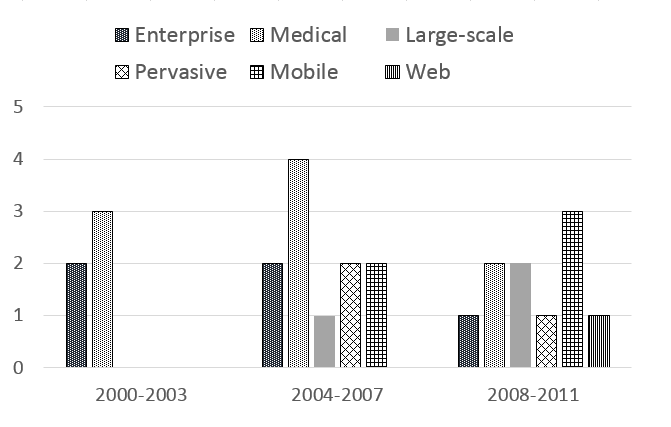
\includegraphics[width=4.0in]{sections/dist_domains_byYear.png}
\vspace{-0.2 in}
    \caption{\label{fig:dist_domains}Domain distribution by 3-year period. Y-axis represents the number of corresponding domain papers.
    X-axis represents 3-year period from 2000 to 2011.}
\end{figure}



The medical domain produced the largest selection of papers when analyzing the domains influencing the proposals of RBAC extension models.  
Moreover, we observed that the categories associated with papers identifying the medical domain were not limited to one or two but cut across
each of the eight categories except for the Organizational category. 
The cross-category nature of the medical domain papers appears indicative of the complex nature of medical applications and the requirements therein.
Given the growth of the research and development of medical applications over the past decade this result does not appear to be surprising. However,
the RBAC standard was originally created to reduce cost and increase interoperability - two goals of current regulation around the standardization
of electronic health record systems. The large number of proposed models, and the cross-category result stand in direct opposition of the goals
of both the RBAC standard and current regulations.

The RBAC standard has been re-enforced by the economic impact that standardization has had on enterprises needing to apply access control.  The
inclusion of extension models targeted at the enterprise workflow domain is indicative of the expansion of requirements for enterprises. Developers
and researchers should take care when looking at extension models designed to address the newer requirements of enterprise workflows in order to
achieve the same economic implementation and maintainability benefits the RBAC Reference Model presents.

Figure~\ref{fig:dist_domains} shows domain distribution by 3-year period.
We observed that medical and enterprise domain papers constantly appear for every period in Figure~\ref{fig:dist_domains}.
For a domain that has roots in medical and enterprise computing, protecting the data of both through access controls is paramount given their ubiquity. 
Mobile computing has seen a dramatic increase in the number of available devices, operating systems and applications since 1997 when the first smart phone was introduced. Since 2004, the domain analysis results produced five papers that targeted extensions that are designed to address the requirements of mobile computing. 



\section{Generalizations} \label{sec:generalizations}

RQ6: What commonalities or generalizations exist across all categories?

\subsection{Results}

The RBAC standard is used in various aspects of computer systems. In order to reduce efforts for modeling access control used in various applications, researchers often focus on developing generalized core concepts of access control.
The authors use propositional logic to describe access control model across all categorizations. Propositional logic is concerned with propositions and their logical relationships. In propositional logic, simple (i.e., atomic) or compound condition at given context is evaluated to true or false based on specified rules and access control logic. Researchers are concerned to extend limited set of propositions specific to core RBAC to meet real-world scenarios such as dynamic constraints, temporal, or spatial constraints. However, semantic meanings of such propositions are various based on researchers' intention.

\subsection{Analysis and Discussion}

Since NIST proposed RBAC standard using propositional logic, researchers describe extended RBAC models using propositional logic. Given context, propositional logic is used to evaluate true or false based on specified rules and access control logic. As access control is typically evaluated to either true or false based on predicates, propositional logic is sufficient to describe key ideas and definitions. We found that 27 papers of RBAC extensions use propositional logic to describe its extended model.
However, propositional logic has limitations. While this logic is simple, this logic does not support for reasoning about RBAC, which helps
reduce the administrative complexity of associations such as user- role associations.
In order to support for reasoning of access control, one may describe the RBAC extended models in first-order logic. 
Given an RBAC extension model, Samuel et al.~\cite{samuel07:spatio-temporal} proposed verification of the model using a specification language, which is based first-order logic. This logic is sufficient to model RBAC and extended RBAC for reasoning. Moreover, this logic supports for concise and elegant formulation of the Reference Model and its relation.  First-Order logic is expressive enough to concisely represent access control systems. First-Order logic uses relations, variables, and quantifiers.
